\chapter{Recurrent Neural Networks}
\label{chap:rnn}
Ein Schwerpunkt dieser Arbeit sind RNN. Diese speziell für die Klassifikation und Regression von sequentiellen Daten entwickelte DNN-Architektur findet besonders in Anwendungsfällen, in denen die Reihenfolge von Daten eine dominante Rolle in der Richtigkeit der Klassifikation spielt, Verwendung. Auch im Bereich der Klassifikation von sEMG-Signalen wurden RNN in der Vergangenheit bereits erfolgreich utilisiert (\cite{simao2019emg}). Trotz der Möglichkeit der Interpretation von sequentiellen Daten ergeben sich bei der Arbeit mit RNN einige Schwierigkeiten (\cite{pascanu2013difficulty}), weshalb das Training solcher Netzwerke nicht immer problemlos verläuft. Insbesondere die \textit{Vanishing Gradient} (VG) und \textit{Exploding Gradient} (EG) Problematiken sind nach \cite{pascanu2013difficulty} typisch und werden im Folgenden ebenfalls beschrieben. Um diese zu umgehen, werden in dieser Arbeit zusätzlich \textit{long short term memory} und \textit{gated recurrent unit} Architekturen verwendet und ebenfalls weiter ausgeführt.

\section{Einführung Recurrent Neural Networks}
\label{sec:rnn}
RNN ähneln nach \cite{pascanu2013difficulty} in ihrer Architektur gewöhnlichen MLP. Im Fall von RNN werden die HL jedoch rekurrent durchlaufen, um aus Sequenzen zu lernen. Das bedeutet, dass ein HL für jeden Input in einer Sequenz einmal durchlaufen wird und der Output des vorherigen Durchlaufs stets zum Input des nächsten Durchlaufs hinzugefügt wird. 

\begin{figure}[h]
    \begin{center}
        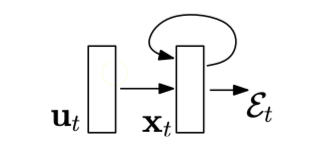
\includegraphics[scale=0.8]{grafiken/rnn-basic.png}
        \caption{Grundlegender Aufbau eines RNN mit Input Layer $u_t$ und HL $x_t$ (\cite{pascanu2013difficulty})}
        \label{rnn-basic}
    \end{center}
\end{figure}

Durch diesen Aufbau können RNN theoretisch Sequenzen beliebiger Länge durchlaufen und diese erlernen (\cite{pascanu2013difficulty}). 

% Mathematischer Aufbau hinzufügen

Um das Training von RNN mit dem aufgezeichneten Datensatz zu ermöglichen, wurden die darin enthaltenen Daten in solche Sequenzen unterteilt. Da es sich hier um ein Problem der Klassifikation handelt und jede Sequenz von Daten einem Ergebnis entspricht, wurden die im Datensatz enthaltenen Aufnahmen für diese Arbeit nach aufeinanderfolgenden Bewegungsklassen gruppiert. Die daraus entstehenden Sequenzen wurden mit der jeweils zugehörigen Klasse gelabelt und anschließend in die Architekturen hineingegeben.

Zunächst wurde ein gewöhnliches RNN untersucht. Hierfür wurde nach händischer Optimierung eine Struktur mit vier HL gewählt. Die ersten drei HL mit je 124 Neuronen waren dabei RNN Schichten, die jeweils die Sequenzen rekurrent durchliefen, bevor die Daten an die vierte Schicht, einen Dense-Layer mit 32 Neuronen und einer Rectifier Linear Unit (ReLU) Aktivierungsfunktion, übergeben wurden. Dieser übergab die Daten an den Output Layer mit elf Neuronen, der nach Durchlaufen einer Softmax Aktivierungsfunktion das Ergebnis der Klassifikation ausgab. Diese Architektur wurde über 100 Epochen mit dem Datensatz trainiert und mittels zehnfacher Cross Validation evaluiert.

Unter der Betrachtung der erzielten Klassifikationsgenauigkeit auf dem Validierungsdatensatz waren die Ergebnisse dieser Architektur zunächst vergleichbar mit der Genauigkeit anderer Klassifikatoren wie dem MLP oder kNN.
So stellte sich nach der 47. Epoche eine Asymptotisierung ein und die Genauigkeit der Klassifikation schwankte nur noch um die 85\% Marke. Dies kann man an Abbildung \ref{srnn-1-acc} erkennen.

\begin{figure}[h]
    \begin{center}
        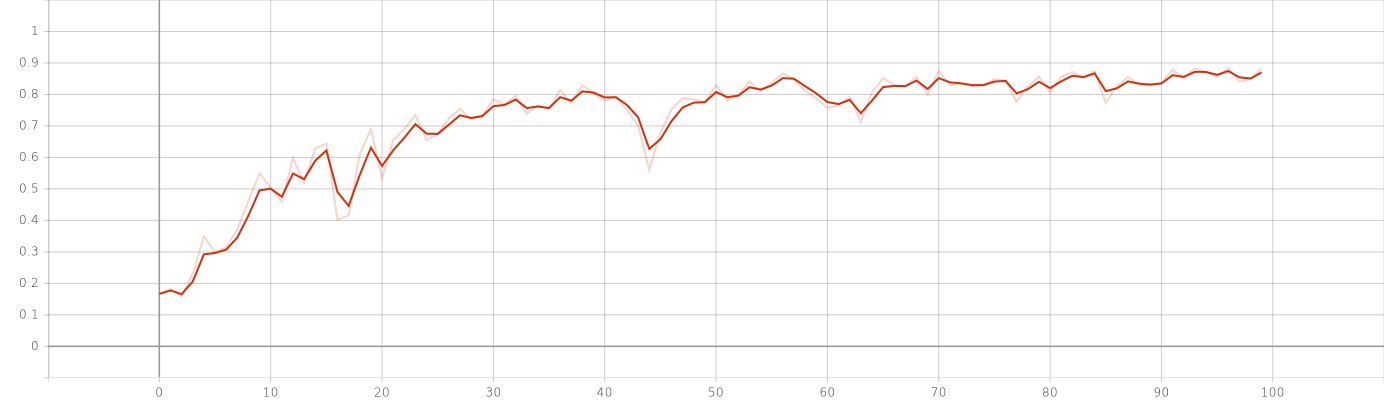
\includegraphics[scale=0.3]{grafiken/srnn-1-acc.png}
        \caption{Darstellung der Genauigkeit auf dem Validierungsdatensatz in Abhängigkeit der Epoche}
        \label{srnn-1-acc}
    \end{center}
\end{figure}

Das untersuchte Netzwerk unterliegt hier allerdings noch einigen Einbußen, die durch Betrachten der Entwicklung des Klassifikationsfehlers in Abhängigkeit der Epoche auffallen. Während diese nämlich im Fall von gewöhnlich lernenden Netzwerken stetig fallen sollte, enthält die Grafik der untersuchten Netzwerkarchitektur große Ausschläge im Verlauf des Trainings (Abbildung \ref{rnn-1-loss}).

\begin{figure}[h]
    \begin{center}
        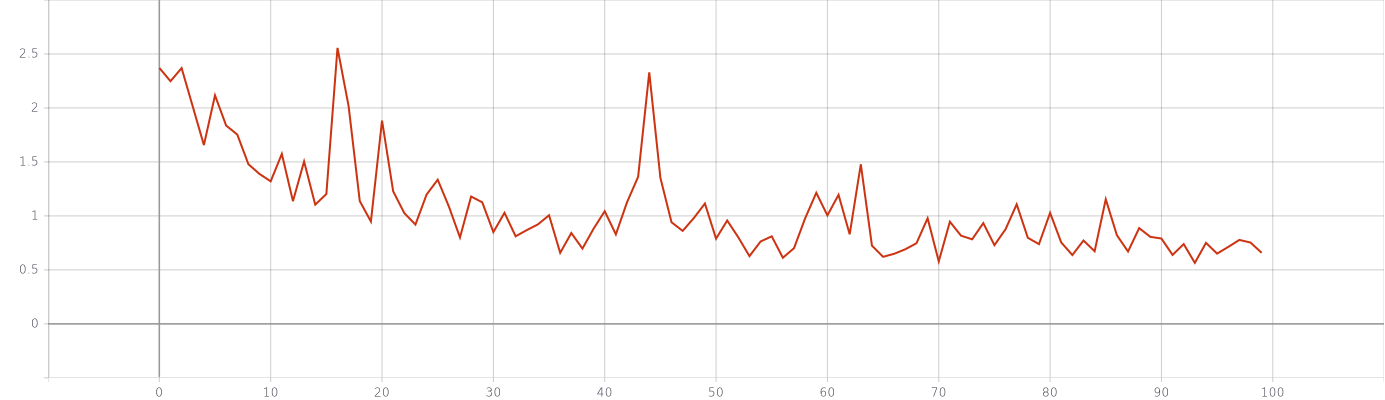
\includegraphics[scale=0.3]{grafiken/rnn-1-loss.png}
        \caption{Klassifikationsfehler der RNN Architektur in Abhängigkeit der Epoche}
        \label{rnn-1-loss}
    \end{center}
\end{figure}

Diese starken Ausschläge im Fehlerwert der Klassifikation deuten nach \cite{pascanu2013difficulty} häufig auf die Problematik eines \textit{Exploding Gradient} hin. Diese entsteht im Kontext von RNN-Architekturen während der Gradientenberechnung in der \textit{Backpropagation Through Time} (BTT) (\cite{werbos1990backpropagation}). Da Neuronale Netze wie in Kapitel 4 dieser Arbeit Informationen durch die Gewichtung einzelner Neuronen speichern (\cite{haykin2007neural}), wird dieser Mechanismus auch in RNN genutzt um Informationen vorheriger Durchläufe der Sequenzen zu speichern (\cite{werbos1990backpropagation}). Somit betrifft BTT nicht nur die Anpassung der Parameter von Layer zu Layer, sondern auch von Sequenzabschnitt zu Sequenzabschnitt (\cite{werbos1990backpropagation}). So wird zur Initialisierung eines Neurons in einem RNN stets der \textit{hidden state} des vorherigen Durchlaufs hinzugefügt und so forwärtspropagiert (\cite{pascanu2013difficulty}). Vor allem bei langen Sequenzen, in denen die Gewichte der Aktivierungsfunktion $w > 1$ entsprechen, kommt es durch die mehrfache Multiplikation der Werte zu sehr hohen Gradientenwerten gegen unendlich, die das Netzwerk mit einem Durchlauf bereits sehr stark beeinflussen. EG sind zwar kein Problem, das sich auf RNN beschränkt, sie sind hier allerdings aufgrund der in diesen angewandten BTT in solchen Architekturen häufiger anzutreffen (\cite{pascanu2013difficulty}).

Eine von \cite{pascanu2013difficulty} angesprochene und in der Praxis häufig angewandte Methode ist die des \textit{gradient clipping} (GC). Hier wird für den Gradienten eine Schwelle festgelegt, auf die er reduziert oder erhöht wird, sollte er diese über- oder unterschreiten. Das begrenzt den Gradienten auf einen bestimmten Wertebereich und unterbindet somit die für EG üblichen starken Ausschläge. Die Verwendung von GC in der untersuchten Architektur führte zu einer mit weniger Ausschlägen verlaufenden Fehler- und Klassifikationsgenauigkeitskurve.

GC glättet zwar den Verlauf des Klassifizierungsfehlers und macht diesen insgesamt weniger volatil, reduziert allerdings ebenfalls die erzielte Klassifizierungsgenauigkeit der Architektur. Während dies aufgrund des stagnierenden Fehlerwertes und somit potenziell stagnierenden Gewichten auf den gegenteiligen Effekt des GC, den \textit{vanishing gradient} (VG), hinweisen könnte, ist das Nachweisen von VG in RNN anhand der vorhandenen Daten schwierig. Um die Schwierigkeiten rund um EG und VG zu umgehen, können die RNN-Architekturen LSTM und GRU verwendet werden (\cite{simao2019emg}), die im Verlauf dieser Arbeit ebenfalls auf den Datensatz angewandt wurden und gute Ergebnisse erzielten.

Zwar erreichte die gewöhnliche RNN-Architektur nach Optimierung und Einsatz von GC eine stabile Klassifikationsgenauigkeit, sie führte allerdings im Hinblick auf die Trainingsdauer und den Vergleich mit einfacheren Klassifikatoren wie dem MLP, kNN oder SVM zu Ergebnissen, die eine praktische Anwendung der Architektur ausschließen würden. Andere Klassifikatoren erreichten hier in einer häufig geringeren Trainingsdauer präzisere Klassifikationsergebnisse, wie in Kapitel 7 dieser Arbeit aufgezeigt wird.


\section{Long Short Term Memory}
\label{sec:lstm}

Während RNN auf gewöhnlichen Feed-Forward-Netzen aufbauen, in dem sie die HL mit Schleifen versehen und dadurch die zeitlichen Beziehungen interpretieren können (\cite{simao2019emg}), haben gewöhnliche RNN Strukturen häufig Probleme bei Sequenzen mit langer Aufnahmespanne (\cite{pascanu2013difficulty}). Typische Konsequenzen sind hier wie obig angesprochen die VG- und EG-Problematik. LSTM-Architekturen lösen dieses Problem, indem sie die Anzahl der Gewichte und Biases eines in einem RNN enthaltenen Neurons vervierfachen. Dadurch erhält das Netzwerk die Möglichkeit, vergangene Informationen durch sogenannte Gates zu filtern (\cite{simao2019emg}). Diese Kombinationen aus Gewicht und Bias ergeben nach \cite{simao2019emg} folgende Gates:

\begin{itemize}
    \item \textit{input gate layer} (IGL)
    \item \textit{forget gate layer} (FGL)
    \item \textit{output gate layer} (OGL)
    \item \textit{state gate layer} (SGL)
\end{itemize}

Der FGL und IGL bestimmen durch ihr Gewicht und Bias, wie der \textit{hidden state} der letzten Sequenz und der aktuelle Input die Aktivierung des aktuellen Neurons beeinflussen. Die nachfolgenden von \cite{simao2019emg} aufgestellten Gleichungen zeigen dies mathematisch auf.

$$i_t=\sigma(W_i*[h_{t-1}, x_t]+b_i)$$
$$f_t=\sigma(W_f*[h_{t-1}, x_t]+b_f)$$

Dabei stellen die mit $i$ indexierten Gewichte und der Bias die trainierbaren Parameter des IGL und die mit $f$ indexierten Parameter die des FGL dar. $t$ steht für die aktuelle zeitliche Sequenz (\cite{simao2019emg}). 

Diese zwei Sigmoid Funktionen ergeben Werte zwischen 0 und 1, die durch Multiplikation mit dem \textit{cell state} (CS) der vorgehenden Periode $c_{t-1}$ und dem vorläufigen CS der neuen Periode $\widetilde{c}_t$ jeweils den Einfluss auf den CS der aktuellen Period $c_t$ steuern. $\widetilde{c}_t$ entspricht dabei, wie in der folgenden Gleichung zu sehen, dem CS eines normalen RNN. Der Einfluss von diesem auf den neuen CS wird hier allerdings durch den IGL geregelt.

$$\widetilde{c}_t=tanh(W_c*[h_{t-1}, x_t]-b_c)$$

Der zum Schluss ausgegebene CS setzt sich somit zusammen aus dem CS der vorigen Periode $c_{t-1}$ und dem vorläufigen CS $\widetilde{c}_t$ der aktuellen Periode, gewichtet mit dem Wert des VGL und des IGL.

$$c_t=f_t*c_{t-1}+i_t*\widetilde{c}_t$$

Durch den OGL wird der an den nächsten Schritt übergebene \textit{hidden state} (HS) gesteuert. So ergibt sich der weitergegebene HS $h_t$ aus dem Ergebnis der OGL $o_t$ multipliziert mit durch die tang-Aktivierungsfunktion normierte CS $c_t$.

$$o_t=\sigma(W_o*[h_{t-1}, x_t]-b_o)$$
$$h_t=o_t*tanh(c_t)$$

Durch diese Gates kann der CS und HS auch über lange Sequenzen hinweg erhalten bleiben. Das führt dazu, dass das Netzwerk lange zurückliegende Abschnitte von Sequenzen nicht vergisst, sondern beibehält und dadurch die Problematiken des VG und EG in gewöhnlichen RNN löst (\cite{simao2019emg}). 

Auch unter Training auf dem in dieser Arbeit verwendeten Datensatz erzielte die LSTM Architektur gute Ergebnisse. Insbesondere im Vergleich mit gewöhnlichen RNN fällt die starke Erhöhung in der Klassifikationsgenauigkeit auf dem Validierungsdatensatz und die schnelle Asymptotisierung desselbigen auf. Auch die Volatilität sowohl des Klassifikationsfehlers als auch der Klassifikationsgenauigkeit in Abhängigkeit der Epoche reduzierte sich, wie in den Abbildungen \ref{lstm-acc} zu sehen, drastisch. Die LSTM-Architektur erzielte nach 100 Epochen eine Klassifikationsgenauigkeit von 98,11\%. Anzumerken ist hierbei allerdings, dass hierfür eine Trainingsdauer von 58 Minuten und 28 Sekunden benötigt wurde, was der höchsten in dieser Forschungsarbeit untersuchten Trainingsdauer entspricht.

\begin{figure}[h]
    \centering
    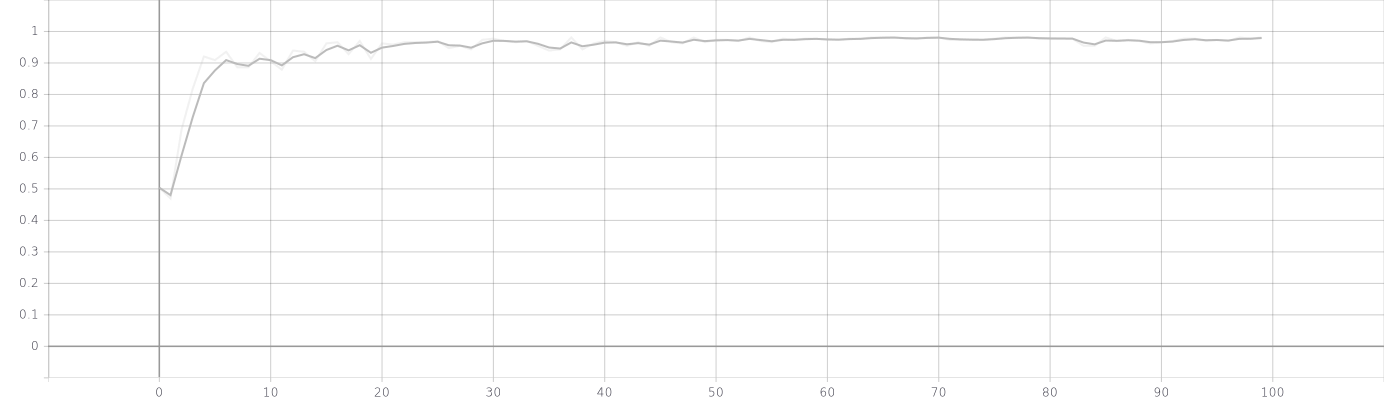
\includegraphics[scale=0.3]{grafiken/lstm-acc.png}
    \caption{Klassifikationsgenauigkeit der verwendeten LSTM Architektur in Abhängigkeit der Epoche auf dem Validierungsdatensatz}
    \label{lstm-acc}
\end{figure}


\section{Gated Recurrent Unit}
\label{sec:gru}

\textit{Gated Recurrent Units} (GRU) wurden durch \cite{cho-etal-2014-learning} mit derselben Intention entwickelt wie LSTM Architekturen und haben daher dieselben Vorteile gegenüber von gewöhnlichen RNN-Architekturen. Allerdings unterscheiden sich GRU in ihrer Funktionsweise und Parameteranzahl nach \cite{simao2019emg} von LSTM Architekturen. So ist ein Vorteil der GRU Architekturen gegenüber LSTM die reduzierte Parameterzahl. Diese führt zu einer schnelleren Trainings- und Klassifikationszeit (\cite{simao2019emg}). Die geringere Parameterzahl erreichen GRU durch eine geringere Anzahl an Gates. Anders als bei LSTM gibt es hier lediglich zwei mit trainierbaren Parametern. Diese sind das \textit{update gate} (UG) $z_t$ und das \textit{reset gate} (RG) $r_t$. Dies lässt sich durch folgende von \cite{simao2019emg} aufgestellten Gleichungen veranschaulichen:

$$z_t=\sigma(W_z*[h_{t-1}, x_t])$$ 
$$r_t=\sigma(W_r*[h_{t-1}, x_t])$$ 

Anders als im Fall von LSTM Architekturen enthalten GRU keinen CS, sondern vermitteln sämtliche sequentielle Daten über den \textit{hidden state} $h_t$ (\cite{simao2019emg}). Das RG bestimmt durch die Funktion von $\widetilde{h}_t$, wie viel der vorherigen Information nicht in den nächsten HS übergeben, also vergessen, werden soll. Dies geschieht durch die Gewichtung des vorigen HS $h_{t-1}$.

$$\widetilde{h}_t=tanh(W*[r_t*h_{t-1}, x_t])$$

Abschließend wird der ausgegebene HS $h_t$ berechnet, indem der vorige HS $h_{t-1}$ und der neue vorläufige HS $\widetilde{h}_t$ mithilfe von dem UG $z_t$ gewichtet werden.

$$h_t=(1-z_t)*h_{t-1}+z_t*\widetilde{h}_t$$

Wie an dem Aufbau der Funktionen von UG und RG zu erkennen, enthalten diese zusätzlich keinen Bias, was zu einer weiter reduzierten Zahl an trainierbaren Parametern beiträgt und somit die Trainings- und Klassifikationsdauer weiter verringert (\cite{simao2019emg}).

Auch in der im Zuge der Forschungsarbeit untersuchten GRU-Architektur ließ sich diese Annahme bestätigen. So ist die GRU Architektur mit einer Trainingsdauer von 18 Minuten und 2 Sekunden die schnellste DNN Architektur in diesem Experiment. Sie erreichte dabei mit einer 98,11\%igen Klassifikationsgenauigkeit dieselbe Präzision wie die LSTM Architektur in einem Drittel der Trainingsdauer.

\begin{figure}[h]
    \centering
    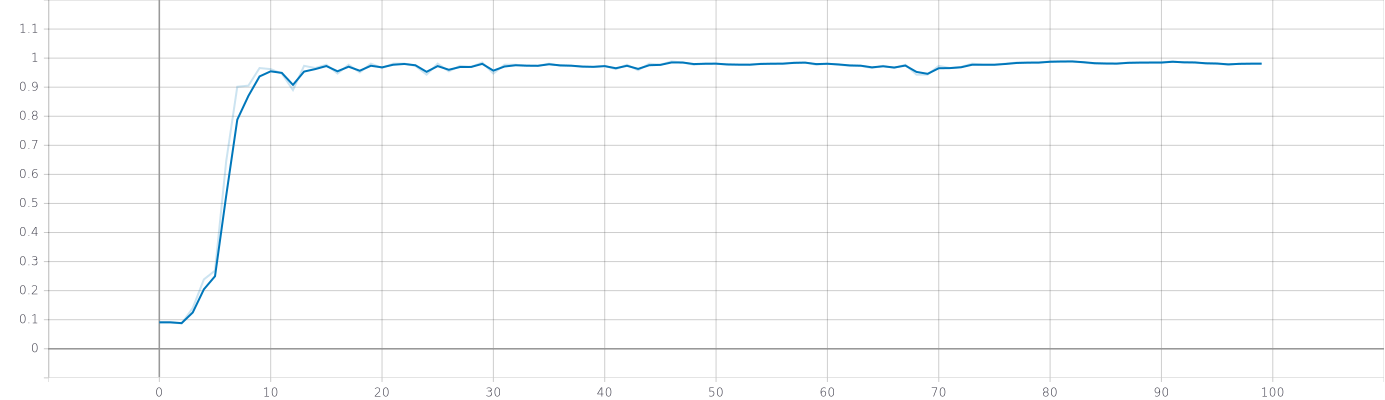
\includegraphics[scale=0.3]{grafiken/gru-acc.png}
    \caption{Klassifikationsgenauigkeit der GRU Architektur auf dem Validierungsdatensatz in Abhängigkeit der Epoche}
    \label{gru-acc}
\end{figure}